
À plus forte raison que pour les dérivées, il est parfois compliqué de calculer
des intégrales analytiques. Dans ce TP, nous écrirons des programmes
calculant numériquement des approximations d'intégrales.

La méthode utilisée est basée sur le théorème fondamental de l'analyse.
Celui-ci faisant le lien entre primitive et intégrale au sens de Riemann :
\begin{equation}
\begin{split}
\int_a^b f(x)dx &= F(b)-F(a) \\
                &= \lim_{n\rightarrow\infty} \sum_{i=0}^{n-1}\frac{(b-a)}{n} f(a+i\frac{(b-a)}{n})\\
                &= \lim_{n\rightarrow\infty} \sum_{i=0}^{n-1} h_n f(x_i)
\end{split}
\end{equation}
Où $dF = f(x)dx$, $h_n=\frac{(b-a)}{n}$, et $x_i=a+ i\frac{(b-a)}{n} = a+ih_n$.

\begin{center}
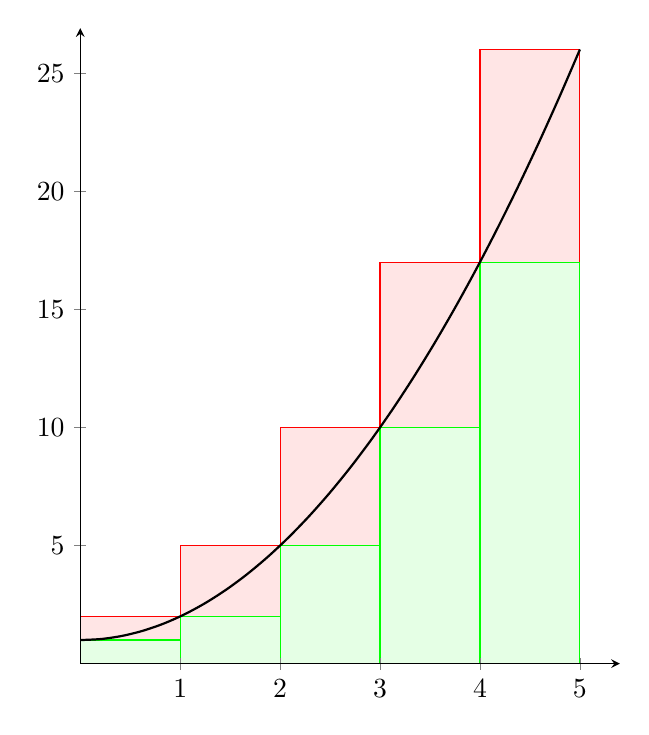
\begin{tikzpicture}
\begin{axis}[
    xtick={0,...,5},ytick={5,10,15,20,25},                    y=0.3cm,
    xmax=5.4,ymax=26.9,ymin=0,xmin=0,     enlargelimits=true,     axis
    lines=middle,  clip=false,  domain=0:5,  axis on  top  ]  \addplot
  [draw=red,fill=red!10,const    plot     mark    right,    samples=6]
  {1+x^2}\closedcycle;   \addplot  [draw=green,   fill=green!10,  ybar
    interval,    samples=6]   {1+x^2}\closedcycle;    \addplot[smooth,
    thick,domain=0:5]{1+x^2};
\end{axis}
\end{tikzpicture}
\end{center}

\subsection{Méthode des rectangles}
\begin{enumerate}
  %%
\item À  partir de  la formule ci-avant,  écrire une  fonction capable
  d'estimer $\int_a^b  f(x)dx$ pour toute fonction  $f(x)$ définie sur
  l'intervalle $[a\,;\,b]$.  La fonction  d'intégration
  à   écrire  aura   pour  arguments   :   $f$,  $a$,   $b$,  et   $n$
  \cf{function.py}.
  %%
\item Écrire la même fonction mais prenant cette fois pour argument la
  valeur de  $h$, plutôt que $n$.  La  fonction commencera par  adapter au  plus juste
  cette valeur à l'intervalle $[a\,;\,b]$ reçu.
  %%
\item Proposer  une nouvelle  fonction utilisant la précédente
  pour calculer  $N$ intégrales de  $a$ à $x$,  où les valeurs  de $x$
  seront  uniformément  réparties  entre  $a$ et  $b$.
  \begin{itemize}
  \item[$\ast$] Cette fonction aura donc  pour arguments $f$, $a$, $b$,
    $N$, et $h$ ;
  \item[$\ast$] elle retournera deux listes :  les valeurs   de  $x$   et
    celles  de   l'intégrale  correspondante $\int_a^xf(t)dt$.
  \end{itemize}
  Tester cette fonction en prenant $f=\cos$, $a=0$, $b=\pi$, $N=100$, et
  $h=0,01$
  \cf{mesh.py, loop.py et returnList.py}.\\
%%
\item  Sur un même graphique, tracer $\int_a^xf(t)dt$ et $\sin(x)$ en fonction de $x$
  \cf{plot.py}.
  %%
\item  Calculer  l'écart  moyen $\varepsilon$ entre  $\int_a^xf(t)dt$  et  $\sin(x)$
  \cf{loop.py}.
  %%
\item  Tracer l'évolution  de  $\varepsilon$  en fonction  de  $h$ sur  un
  graphique   log/log. Utiliser  des valeurs  de  $h$  appartenant à  une  suite
  géométrique de  raison 4 et  de valeur initiale $10^{-4}$.  Faire le
  tracé pour des valeurs de $h$ allant jusqu'à $10^{-2}$.
  %%
\item Aux   mêmes  points   tracer  $f(x)=x$,   puis  comparer.


\end{enumerate}

\subsection{Intervalle de confiance}
Pour une fonction strictement croissante  sur un intervalle, le calcul
précédent  est une  minoration  de l'intégrale \footnote{Et inversement pour  une
fonction strictement décroissante}. À  partir de cette constatation, il
est  possible   d'écrire  un  programme  donnant   un  encadrement  de
l'intégrale d'une fonction.
\begin{enumerate}
  %%
\item Écrire deux fonctions calculant :
  \begin{eqnarray*}
    \sum_{i=1}^n h_n f(x_i)\\ \sum_{i=0}^{n-1}h_n f(x_i)
  \end{eqnarray*}
  Ces méthodes sont appelées,  respectivement, méthodes des rectangles
  à droite et  à gauche.  \\ Comparer les  intégrations réalisées avec
  ces deux méthodes.

  %%
\item  Vérifier  sur  quelques  exemples  que  pour  des  portions  de
  fonction monotone, l'une des  intégrations donne une majoration de
  l'intégrale alors que l'autre donne une minoration.  %%
\item Écrire  une fonction  calculant simultanément une  majoration et
  une       minoration        approximative       de       l'intégrale
  \cf{if.py}.\\ L'algorithme sera le suivant :
  \begin{itemize}
  \item[$\ast$]  Pour  chaque  pas   d'intégration  $h$,  calculer  la
    fonction à droite puis à gauche ;
  \item[$\ast$] comparer les deux valeurs obtenues pour le terme $h\,f$ ;
  \item[$\ast$] utiliser la plus petite pour évaluer la minoration ;
  \item[$\ast$] employer la plus grande pour calculer la majoration.
\end{itemize}
\end{enumerate}

\subsection{Méthodes d'ordre plus élevé {\sc[Facultatif]}}

%%https://perso.univ-rennes1.fr/marie-pierre.lebaud/agint/ecrit/analyse-reelle/integration-numerique/X-int-num.pdf

Il est possible d'approximer l'intégrale d'une fonction par des
méthodes plus efficaces.
\begin{enumerate}
\item La  première consiste  à calculer non  pas l'aire  de rectangles
  sous/sur la courbe, mais celle de trapèzes.
  \begin{equation}
    \begin{split}
      \int_a^b        f(x)dx       &\simeq        \sum_{i=0}^{n-1}       h_n
      \frac{(f(x_i)+f(x_{i+1})}{2}\\ &\simeq \frac{h_n}{2} \left(f(a)+f(b) +
      2\sum_{i=1}^{n-1} f(x_i) \right).
    \end{split}
  \end{equation}
  \begin{itemize}
  \item[$\ast$] Programmer  cette  méthode dans une fonction en parallèle de la précédente
    (c.-à-d. méthode des rectangles).
  \item[$\ast$] Pour la fonction $G(x) = \int_{\sqrt{2}}^{\sqrt{7}} \exp(x) dx$,
    comparer le résultat de l'integration numérique (avec les deux méthodes) à celui de la résolution analytique.
  \item[$\ast$] Calculer et tracer (sur  un graphique  log/log) l'écart $\varepsilon$ entre la méthode numérique
    et la résolution analytique en   fonction  des  valeurs   de  $h$.
  \end{itemize}


\item La méthode d'ordre directement  supérieur est appelée méthode de
  Simpson  composite.  Elle  consiste  à calculer  l'aire sous  chaque
  intervalle comme l'aire  de la parabole passant par  les deux points
  aux extrémités et le point du milieu :
  \begin{equation}
    \int_a^b   f(x)dx  \simeq   \frac{h}{6}\sum_{i=0}^{n-1}  f(x_i)   +  4
    f(x_{i+1/2}) + f(x_{i+1}) .
  \end{equation}

  Programmer  cette méthode  et  comparer sa  précision  en fonction  du
  nombre d'évaluations de la fonction à celle des autres.
\item  Afin de minimiser les évaluations de la fonction à intégrer il est
possible d'obtenir la formulation suivante pour la méthode de Simpson :
 \begin{equation}
\begin{split}
\int_a^b  f(x)dx   \simeq  \frac{h}{48}  &\biggl[17f(a)   +  59f(a+h)+
  43f(a+2h)+
  49f(a+3h)\biggr.\\ &+48\sum_{i=4}^{n-4}f(x_i)\\ &\biggl.+49f(b-3h)+43f(b-2h)+59f(b-h)+17f(b)\biggr]
\end{split}
 \end{equation}

 Ajouter cette formulation à votre  comparatif en faisant attention au fait
 qu'elle ne peut être utilisée pour $n<8$.
\item  Les quadratures  de Gauss-Legendre  consistent à  approximer la
  fonction à  intégrer par un  polynôme de  Legendre. Il en  existe de
  divers degrés  $m$, où $m$  est aussi  le nombre d'évaluations  de la
  fonction sur  l'intervalle d'intégration.   Elles sont  exactes pour
  l'intégration de  polynômes de  degrés $2m+1$.  Pour réussir  un tel
  exploit, il faut choisir des  points bien particuliers où évaluer la
  fonction :
\begin{center}
\begin{tabular}{ccc}
Ordre $m$& Points $p_j$ &Pondération $w_j$\\
\hline\hline
\strut$1$ & $0$ & $2$ \\\hline
\strut$2$ & $\pm \sqrt{1/3}$ & 1\\\hline
\multirow{2}{*}{$3$} &  $0$              & $8/9$\\
                     & $\pm\sqrt{3/5}$   & $5/9$\\\hline
\multirow{2}{*}{$4$} &  $\pm\sqrt{\frac{3}{7}-\frac{2}{7}\sqrt{\frac{6}{5}}}$              & $\frac{18+\sqrt{30}}{36}$\\
                     &  $\pm\sqrt{\frac{3}{7}+\frac{2}{7}\sqrt{\frac{6}{5}}}$              & $\frac{18-\sqrt{30}}{36}$\\\hline
\multirow{3}{*}{$5$} & $0$ & $\frac{128}{225}$\\
                     &  $\pm\frac{1}{3}\sqrt{5-2\sqrt{\frac{10}{7}}}$ & $\frac{322+13\sqrt{70}}{900}$\\
                     &  $\pm\frac{1}{3}\sqrt{5+2\sqrt{\frac{10}{7}}}$ & $\frac{322-13\sqrt{70}}{900}$\\

\end{tabular}
\end{center}
Ces  approximations  sont  plutôt  destinées  à  être  employées  pour
calculer     une     intégrale    sans     subdiviser     l'intervalle
d'intégration.  Nonobstant en  opérant  la subdivision,  on obtient  la
formule :
\begin{equation}
\int_a^b   f(x)dx   \simeq   \sum_{i=0}^{n-1}   \sum_{j=0}^{m-1}   w_j
f(x_i+\frac{h}{2}(1+p_j))
\end{equation}
Comparer  ces  quadratures  aux autres  intégrateurs  déjà  programmés.\\
\cf{listElement.py et listOfList.py}





\end{enumerate}
